% README file for moduleDocumentationTemplate TeX template.
% This template should be used to document all Basilisk modules.
% Updated 20170711 - S. Carnahan
%
%-Copy the contents of this folder to your own _Documentation folder
%
%-Rename the Basilisk-moduleDocumentationTemplate.tex appropriately
%
% All edits should be made in one of:
% sec_modelAssumptionsLimitations.tex
% sec_modelDescription.tex
% sec_modelFunctions.tex
% sec_revisionTable.tex
% sec_testDescription.tex
% sec_testParameters.tex
% sec_testResults.tex
% sec_user_guide.tex
%
%-Some rules about referencing within the document:
%1. If writing the suer guide, assume the module description is present
%2. If writing the validation section, assume the module features section is present
%3. Make no other assumptions about any sections being present. This allow for sections of the document to be used elsewhere without breaking.

%In order to import some of these sections into a document in a different directory:
%\usepackage{import}
%Then, the sections are called with \subimport{relative path}{file} in order to \input{file} using the right relative path.
%\import{full path}{file} can also be used if absolute paths are preferred over relative paths.

%%%%%%%%%%%%%%%%%%%%%%%%%%%%%%%%%%%%%%%%%%%%%%%%%




\documentclass[]{BasiliskReportMemo}

\usepackage{cite}
\usepackage{AVS}
\usepackage{float} %use [H] to keep tables where you put them
\usepackage{array} %easy control of text in tables
\usepackage{graphicx}
\bibliographystyle{plain}


\newcommand{\submiterInstitute}{Autonomous Vehicle Simulation (AVS) Laboratory,\\ University of Colorado}


\newcommand{\ModuleName}{opNavPoint}
\newcommand{\subject}{Pointing using a Camera-Relative OpNav Direction and Rate Gyro Information}
\newcommand{\status}{Released}
\newcommand{\preparer}{T. Teil}
\newcommand{\summary}{This module provides the attitude guidance output for an opNav pointing mode. Typically this would be to point to a planet center, or a specific heading determined from a camera. The input is an optical navigation direction vector, as well as the body rate information.  The output is the standard BSK attitude reference state message.  The target direction measurement is crossed with the desired camera axis that is to point at the sun to create a principle rotation vector.  The dot product between these two vectors is used to extract the principal rotation angle.  With these, a tracking error MRP state is computed.  The body rate tracking errors, relative to the inertial frame, are set equal to the measured body rates to bring the vehicle to rest when pointing at the target.  Thus, the reference angular rate and acceleration vectors relative to the inertial frame are nominally set to zero.  If no heading is available, then the reference rate is set to a camera-fixed value while the attitude tracking error is set to zero.}

\begin{document}

\makeCover

%
%	enter the revision documentation here
%	to add more lines, copy the table entry and the \hline, and paste after the current entry.
%
\newpage
\pagestyle{empty}
{\renewcommand{\arraystretch}{2}
\noindent
\begin{longtable}{|p{0.5in}|p{3.5in}|p{1.07in}|p{0.9in}|}
\hline
{\bfseries Rev} & {\bfseries Change Description} & {\bfseries By}& {\bfseries Date} \\
\hline
1.0 & First Documentation of this module: Nearly Identical to sunSafePoint & T. Teil & 2019-09-01\\
\hline

\end{longtable}
}


\setcounter{page}{1}
\pagestyle{fancy}

\tableofcontents %Autogenerate the table of contents
~\\ \hrule ~\\ %Makes the line under table of contents










	
% !TEX root = ./Basilisk-celestialTwoBodyPoint-20190311.tex

\section{Model Description}


\subsection{Module Goal}
This module computes a reference whose aim is to track the center of a primary target, e.g. pointing the communication antenna at the Earth, at the same time of trying to meet a secondary constraint as best as possible, e.g. a solar panel normal axis pointing the closest in the direction of the Sun.  It is important to note that two pointing conditions in a three-dimensional space compose an overdetermined problem. Thus, the main constraint is always priorized over the secondary one so the former can always be met.\\
Figure~\ref{fig:fig1} shows the case where Mars is the primary celestial body and the Sun is the secondary one. Note that the origin of the desired reference frame $\mathcal{R}$ is the position of the spacecraft.
\begin{figure}[htb]
	\centerline{
	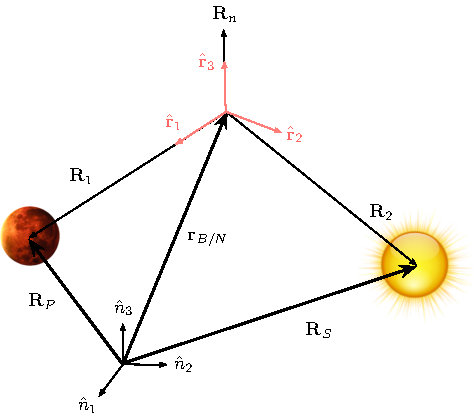
\includegraphics[]{Figures/fig1.pdf}
	}
	\caption{Illustration of the restricted two-body pointing reference frame $\mathcal{R}:\{ \hat{\bm r}_{1},\hat{\bm r}_{1}, \hat{\bm r}_{2} \}$ and the inertial frame $\mathcal{N}:\{ \hat{\bm n}_{1},\hat{\bm n}_{1}, \hat{\bm n}_{2} \}$.}
	\label{fig:fig1}
\end{figure}

Assuming knowledge of the position of the spacecraft $\bm{r}_{B/N}$ and the involved celestial bodies, $\bm{R}_{P1}$ and  $\bm{R}_{P2}$ (all of them relative to the inertial frame $\mathcal{N}$ and expressed in inertial frame components), the relative position of the celestial bodies with respect to the spacecraft is obtained by simple subtraction:
\begin{subequations}
	\begin{align}
		 \bm{R}_{P1} =\bm{R}_{P} - \bm{r}_{B/N} \\
		 \bm{R}_{P2} =\bm{R}_{S} - \bm{r}_{B/N} 
	\end{align}
\end{subequations}

In analogy, the inertial derivatives of these position vectors are obtained:
\begin{subequations}
	\begin{align}
		 \bm{v}_{P1} &=\bm{v}_{P} - \bm{v}_{B/N} \\
		 \bm{v}_{P2} &=\bm{v}_{S} - \bm{v}_{B/N} \\
		 \bm{a}_{P1} &=\bm{a}_{P} - \bm{a}_{B/N} \\
		 \bm{a}_{P2} &=\bm{a}_{S} - \bm{a}_{B/N} 
	\end{align}
\end{subequations}

The normal vector $\bm{R}_{n}$ of the plane defined by $\bm{R}_{P1}$ and $\bm{R}_{P2}$ is computed through:
\begin{equation}
	\bm R_{n} =\bm{R}_{P1} \times \bm{R}_{P2}
\end{equation}
The inertial time derivative of $\bm{R}_n$ is found using the chain differentiation rule:
\begin{equation}
	\bm {v}_{n} = \bm{v}_{P1} \times \bm{R}_{P2} + \bm{R}_{P1} \times \bm{v}_{P2} 
\end{equation}
And the second time derivative:
\begin{equation}
	\bm {a}_{n} = \bm{a}_{P1} \times \bm{R}_{P2} + \bm{R}_{P1} \times \bm{a}_{P2}  + 2 \bm{v}_{P1} \times \bm{v}_{P2} 
\end{equation}
\subsection{ Special Case: No Secondary Constraint Applicable}
If there is no incoming message with a secondary celestial body pointing condition or if the constrain is not valid, an artificial three-dimensional frame is defined instead. Note that a single condition pointing leaves one degree of freedom, hence standing for an underdetermined attitude problem. A secondary constrain is considered to be invalid if the angle between $\bm{R}_{P1}$ and $\bm{R}_{P2}$ is, in absolute value, minor than a set threshold. This could be the case where the primary and secondary celestial bodies are aligned as seen by the spacecraft. In such situation, the primary pointing axis would already satisfy both the primary and the secondary constraints.

Since the main algorithm of this module, which is developed in the following sections, assumes two conditions, the second one is arbitrarily set as following:
\begin{equation}
	\bm{R}_{P2} = \bm{R}_{P1} \times \bm{v}_{P1} \equiv  \bm{h}_{P1}
\end{equation}
By setting the secondary constrain to have the direction of the angular momentum vector $ \bm{h}_{P1}$, it is assured that it will always be valid ($\bm{R}_{P1}$ and $\bm{R}_{P2}$ are now perpendicular).
The first and second time derivatives are steadily computed:
\begin{equation}
	\bm{v}_{P2} =  \bm{R}_{P1} \times \bm{a}_{P1} 
\end{equation}
\begin{equation}
	\bm{a}_{P2} =  \bm{v}_{P1} \times \bm{a}_{P1} 
\end{equation}
\subsection{Reference Frame Definition}
As illustrated in Figure~\ref{fig:fig1}, the base vectors of the desired reference frame $\mathcal{R}$  are defined as following:
\begin{subequations}
	\begin{align}
		\hat{\bm r}_{1} &= \frac{{\bm R}_{P1}} {|{\bm R}_{P1}|} \\
		\hat{\bm r}_{3} &= \frac{{\bm R}_{n}}{|{\bm R}_{n}|} \\
		\hat{\bm r}_{2} &=  \hat{\bm r}_{3} \times \hat{\bm r}_{1} 
	\end{align}
\end{subequations}
Since the position vectors are given in terms of inertial $\mathcal{N}$-frame components, the DCM from the inertial frame $\mathcal{N}$ to the desired reference frame $\mathcal{R}$ is:
\begin{equation}
	[RN] = \begin{bmatrix}
		\leftexp{N}{ \hat{\bm r}_{1}^{T} } \\
		\leftexp{N}{ \hat{\bm r}_{2}^{T} }  \\
		\leftexp{N}{ \hat{\bm r}_{3}^{T} }  
	\end{bmatrix}
\end{equation}
\subsection{Base Vectors Time Derivatives}
The first and second time derivatives of the base vectors that compound the reference frame $\mathcal{R}$ are needed in the following sections to compute the reference angular velocity and acceleration. Several lines of algebra lead to the following sets:
\begin{subequations}
	\begin{align}
		\dot{\hat{\bm{r}}}_1 &= ([I_{3\times3}] - {\hat{\bm{r}}_1}{\hat{\bm{r}}_1}^T)  \frac{{\bm R}_{P1}} {|{\bm R}_{P1}|} \\
		\dot{\hat{\bm{r}}}_3 &= ([I_{3\times3}] - \hat{\bm{r}}_3 \hat{\bm{r}}_3^T)  \frac{{\bm R}_{n}} {|{\bm R}_{n}|} \\
		\dot{\hat{\bm{r}}}_2 &= \dot{\hat{\bm{r}}}_3 \times \bm{r}_1 +  \bm{r}_1  \times \dot{\hat{\bm{r}}}_3 
	\end{align}
\end{subequations}

Steps of the derivation for the first term are given here:

\begin{subequations}
	\begin{align}
		\dot{\hat{\bm{r}}}_1 &= {\bm R}_{P1} \left( {\bm R}_{P1} \cdot {\bm R}_{P1} \right)^{-\frac{1}{2}} \\
		 &= \frac{\dot{\bm R}_{P1}}{|{\bm R}_{P1}|} -  \frac{1}{2} {\bm R}_{P1} {\bm R}_{P1}\cdot \dot{\bm R}_{P1} \left({\bm R}_{P1} \cdot {\bm R}_{P1} \right)^{-\frac{3}{2}} \\
		 &= \frac{\dot{\bm R}_{P1}}{|{\bm R}_{P1}|} -  \hat{\bm r}_1 \hat{\bm r}_{1}^T \frac{\dot{\bm R}_{P1}}{|{\bm R}_{P1}|} \\
		 &=([I_{3\times3}] - {\hat{\bm{r}}_1}{\hat{\bm{r}}_1}^T)  \frac{{\bm R}_{P1}}{|{\bm R}_{P1}|}
	\end{align}
\end{subequations}

The second equation follows an equivalent definition, while the third one completes the frame. The accelerations are given in the following equations:
\begin{subequations}
	\begin{align}
		\ddot{\hat{\bm{r}}}_1 &=  \frac{1}{|{\bm R}_{P1}|}\left(([I_{3\times3}] - {\hat{\bm{r}}_1}{\hat{\bm{r}}_1}^T)  \bm{a}_{P1} - \left(2\dot{\hat{\bm{r}}}_1 \hat{\bm{r}}_1^T  - \hat{\bm{r}}_1 \dot{\hat{\bm{r}}}_1^T \right)  \bm{v}_{P1} \right) \\
		\ddot{\hat{\bm{r}}}_3 &= \frac{1}{|{\bm R}_{n}|}
		\left(
		([I_{3\times3}] - {\hat{\bm{r}}_3}{\hat{\bm{r}}_3}^T)  \bm{a}_{n} - \left(
		2\dot{\hat{\bm{r}}}_3 \hat{\bm{r}}_3 ^T - 
		\hat{\bm{r}}_3 \dot{\hat{\bm{r}}}_3^T \right) \bm{v}_{n}\right) 
		 \\
		\ddot{\hat{\bm{r}}}_2 &= \ddot{\hat{\bm{r}}}_3 \times \bm{r}_1 +  \bm{r}_1  \times \ddot{\hat{\bm{r}}}_3 + 2\dot{\hat{\bm{r}}}_3 \cdot \dot{\hat{\bm{r}}}_1
	\end{align}
\end{subequations}

Elements of the derivation for the first term follow:

\begin{subequations}
	\begin{align}
		\ddot{\hat{\bm{r}}}_1 &= ([I_{3\times3}] - {\hat{\bm{r}}_1}{\hat{\bm{r}}_1}^T) \left(  \frac{\ddot{\bm R}_{P1}}{|{\bm R}_{P1}|} -  \frac{\dot{\bm R}_{P1}}{|{\bm R}_{P1}|}  \frac{\dot{\bm R}_{P1}}{|{\bm R}_{P1}|} ^T \hat{\bm{r}}_1\right)  - \left(\dot{ \hat{\bm{r}}}_1  \hat{\bm{r}}_1^T +  \hat{\bm{r}}_1 \dot{ \hat{\bm{r}}}_1^T\right)\frac{\dot{\bm R}_{P1}}{|{\bm R}_{P1}|}  \\
		&= ([I_{3\times3}] - {\hat{\bm{r}}_1}{\hat{\bm{r}}_1}^T) \frac{\ddot{\bm R}_{P1}}{|{\bm R}_{P1}|} - \left( ([I_{3\times3}] - {\hat{\bm{r}}_1}{\hat{\bm{r}}_1}^T) \frac{\dot{\bm R}_{P1}}{|{\bm R}_{P1}|} \right) \frac{\dot{\bm R}_{P1}}{|{\bm R}_{P1}|} ^T \hat{\bm{r}}_1  - \left(\dot{ \hat{\bm{r}}}_1  \hat{\bm{r}}_1^T +  \hat{\bm{r}}_1 \dot{ \hat{\bm{r}}}_1^T\right)\frac{\dot{\bm R}_{P1}}{|{\bm R}_{P1}|}  \\
		&= ([I_{3\times3}] - {\hat{\bm{r}}_1}{\hat{\bm{r}}_1}^T) \frac{{\bm a}_{P1}}{|{\bm R}_{P1}|} - \dot{ \hat{\bm{r}}}_1 \frac{{\bm v}_{P1}}{|{\bm R}_{P1}|} ^T \hat{\bm{r}}_1  - \left(\dot{ \hat{\bm{r}}}_1  \hat{\bm{r}}_1^T +  \hat{\bm{r}}_1 \dot{ \hat{\bm{r}}}_1^T\right)\frac{{\bm v}_{P1}}{|{\bm R}_{P1}|}  \\
		&= \frac{1}{|{\bm R}_{P1}|}(([I_{3\times3}] - {\hat{\bm{r}}_1}{\hat{\bm{r}}_1}^T)  \bm{a}_{P1} - 2\dot{\hat{\bm{r}}}_1 (\hat{\bm{r}}_1 \cdot \bm{v}_{P1}) - \hat{\bm{r}}_1 (\dot{\hat{\bm{r}}}_1 \cdot \bm{v}_{P1}) ) \\
		&= \frac{1}{|{\bm R}_{P1}|}\left(([I_{3\times3}] - {\hat{\bm{r}}_1}{\hat{\bm{r}}_1}^T)  \bm{a}_{P1} - \left(2\dot{\hat{\bm{r}}}_1 \hat{\bm{r}}_1^T  - \hat{\bm{r}}_1 \dot{\hat{\bm{r}}}_1^T \right)  \bm{v}_{P1} \right)
	\end{align}
\end{subequations}



\subsection{Angular Velocity and Acceleration Descriptions}
Developing some more mathematics, the following elegant expressions of $\bm\omega_{R/N}$ and $\dot{\bm\omega}_{R/N}$ are found:
\begin{subequations}
	\begin{align}
		\bm\omega_{R/N} \cdot \hat{\bm r}_{1}  = \hat{\bm r}_{3} \cdot \dot{\hat{\bm r}}_{2}  \\
		\bm\omega_{R/N} \cdot \hat{\bm r}_{2} = \hat{\bm r}_{1} \cdot \dot{\hat{\bm r}}_{3}\\
		\bm\omega_{R/N} \cdot \hat{\bm r}_{3} = \hat{\bm r}_{2} \cdot \dot{\hat{\bm r}}_{1}
	\end{align}
\end{subequations}
\begin{subequations}
	\begin{align}
		\dot{\bm\omega}_{R/N} \cdot \hat{\bm r}_{1} &=  
		\dot{\hat{\bm r}}_{3} \cdot \dot{\hat{\bm r}}_{2} + \hat{\bm r}_{3} \cdot \ddot{\hat{\bm r}}_{2} -  \bm\omega_{R/N} \cdot \dot{\hat{\bm r}}_{1}
		\\
		\dot{\bm\omega}_{R/N} \cdot \hat{\bm r}_{2} &= 
		 \dot{\hat{\bm r}}_{1} \cdot \dot{\hat{\bm r}}_{3} + \hat{\bm r}_{1} \cdot \ddot{\hat{\bm r}}_{3} -  \bm\omega_{R/N} \cdot \dot{\hat{\bm r}}_{2}	
		\\
		\dot{\bm\omega}_{R/N} \cdot \hat{\bm r}_{3} &=  
		\dot{\hat{\bm r}}_{2} \cdot \dot{\hat{\bm r}}_{1} + \hat{\bm r}_{2} \cdot \ddot{\hat{\bm r}}_{1} -  \bm\omega_{R/N} \cdot \dot{\hat{\bm r}}_{3}
	\end{align}
\end{subequations}
Note that $\bm\omega_{R/N} \cdot \hat{\bm r}_{1}$ is the first component of the angular velocity of the reference with respect to the inertial expressed in reference frame components. Hence,
\begin{equation}
	\bm\omega_{R/N}= \leftexp{R}{
		\begin{bmatrix}
			\bm\omega_{R/N} \cdot \hat{\bm r}_{1} \\
			\bm\omega_{R/N} \cdot \hat{\bm r}_{2}  \\
			\bm\omega_{R/N} \cdot \hat{\bm r}_{3} 
		\end{bmatrix}
	}
\end{equation}
Similarly for the angular acceleration:
\begin{equation}
	\bm{\dot\omega}_{R/N} = \leftexp{R}{
		\begin{bmatrix}
			\bm{\dot\omega}_{R/N} \cdot \hat{\bm r}_{1} \\
			\bm{\dot\omega}_{R/N} \cdot \hat{\bm r}_{2}  \\
			\bm{\dot\omega}_{R/N} \cdot \hat{\bm r}_{3} 
		\end{bmatrix}
	}
\end{equation}
Eventually, in inertial frame components:
\begin{subequations}
	\begin{align}
		\leftexp{N} {\bm\omega_{R/N}} &= [RN] \textrm{ } \leftexp{R} {\bm\omega_{R/N}} 
		\\
		\leftexp{N} {\bm{\dot\omega}_{R/N}} &= [RN]  \textrm{ } \leftexp{R} {\bm{\dot\omega}_{R/N}}
	\end{align}
\end{subequations}

 
  %This section includes mathematical models, code description, etc.

\section{Model Functions}
This section will contain a bullet-list and descriptions of what functions this module performs. For example:
\begin{itemize}
	\item \textbf{computeField()}: The gravity effector module computes the gravity field from a celestial body including spherical harmonics.
	\item \textbf{computeField()}: The gravity effector module computes the gravity field from a celestial body including spherical harmonics.
\end{itemize}

\section{Model Assumptions and Limitations}
This section should describe the assumptions used in formulating the mathematical model and how those assumptions limit the usefulness of the module. %This includes a concise list of what the module does. It also includes model assumptions and limitations

% !TEX root = ./Basilisk-sunSafePoint-20180427.tex

\section{Test Description and Success Criteria}
The mathematics in this module are straight forward and can be tested in a series of input and output evaluation tests.


\subsection{Check 1}
Here a check is performed where the sun vector measurement $\bm s$ has a non-zero length and is not aligned with $\hat{\bm s}_{c}$.  

\subsection{Check 2}
The sun direction vector $\bm s$ is given a norm value that is less than {\tt minUnitMag}.  In this case the attitude tracking $\bm\sigma_{B/R}$ should be set to zero.  Further, the body rate errors are now evaluated relative to a fixed $\bm\omega_{R/N}$ vector.  

\subsection{Check 3}
The sun direction vector $\bm s$ aligned with $\hat{\bm s}_{c}$.  In this case the attitude tracking $\bm\sigma_{B/R}$ should be set to zero.  Further, the body rate errors are simply the inertial body angular rates.  

\subsection{Check 4}
The sun direction vector $\bm s \approx -\hat{\bm s}_{c}$.  In this case the attitude tracking $\bm\sigma_{B/R}$ should be set to $\hat{\bm e}_{180}$.  Further, the body rate errors are simply the inertial body angular rates.  

\subsection{Check 4}
The sun direction vector $\bm s \approx -\hat{\bm s}_{c}$, but $\hat{\bm s}_{c} = \hat{\bm b}_{1}$.  In this case the attitude tracking $\bm\sigma_{B/R}$ should be set to $\hat{\bm e}_{180}$ that is evaluated with the cross product with $\hat{\bm b}_{2}$.  Further, the body rate errors are simply the inertial body angular rates.  


\section{Test Parameters}
The unit test verify that the module output guidance message vectors match expected values.
\begin{table}[htbp]
	\caption{Error tolerance for each test.}
	\label{tab:errortol}
	\centering \fontsize{10}{10}\selectfont
	\begin{tabular}{ c | c } % Column formatting, 
		\hline\hline
		\textbf{Output Value Tested}  & \textbf{Tolerated Error}  \\ 
		\hline
		$\bm\sigma_{B/R}$        & \input{AutoTex/toleranceValue}	   \\ 
		$\bm\omega_{B/R}$        & \input{AutoTex/toleranceValue}\\ 
		$\bm\omega_{R/N}$        & \input{AutoTex/toleranceValue} \\ 
		$\dot{\bm\omega}_{R/N}$        & \input{AutoTex/toleranceValue}  \\ 
		\hline\hline
	\end{tabular}
\end{table}

The nominal module test input values are $\hat{\bm s}_{c} = (0,0,1)$, $\bm s = (1,0,0)$ and $\leftexp{B}{\bm\omega}_{B/N} = (0.01, 0.50, -0.20)$ rad/sec.  The nominal body-fixed search rate is set to $\leftexp{B}{\bm\omega}_{R/N} = (0.0, 0.0, 0.1)$ rad/sec.  This rate is only used if no sun direction vector is available.  The small angle is set to $\epsilon$ = 0.01 degrees.  



\section{Test Results}

All of the tests passed:
\begin{table}[H]
	\caption{Test results}
	\label{tab:results}
	\centering \fontsize{10}{10}\selectfont
	\begin{tabular}{c | c  } % Column formatting, 
		\hline\hline
		\textbf{Check} 						  		&\textbf{Pass/Fail} \\ 
		\hline
	   1	   			& \input{AutoTex/passFail1} \\ 
	   2	   			& \input{AutoTex/passFail2} \\ 
	   3	   			& \input{AutoTex/passFail3} \\ 
	   4	   			& \input{AutoTex/passFail4} \\ 
	   5	   			& \input{AutoTex/passFail5} \\ 
	   \hline\hline
	\end{tabular}
\end{table}



 % This includes test description, test parameters, and test results

\section{User Guide}
For the best examples of the using the Gauss Markov utility, please see the IMU unit test and .cpp files. For other examples, see the simple navigation unit and coarse sun sensor. % Contains a discussion of how to setup and configure  the BSK module






\bibliography{bibliography} %This includes references used and mentioned.

\end{document}
